\section{Komponenten}
\label{section:cganwendung}

\subsection{Module}

Das Framework besteht aus folgenden Modulen

\begin{itemize}
\item \textbf{graphics_core:} Szenengraph (siehe Abschnitt \ref{sec:scene_graph}), Interfaces f�r die Bausteine (Anwendung, UI und Rendering), Picking-Funktionalit�t, Kamera, Datenstrukturen und Algorithmen, I/O, Material
\item \textbf{rendering_jogl:} Rendering mit OpenGL (hier JOGL)
\item \textbf{apps:} Programme, die die Grafik-Funktionalit�t verwenden 
\item \textbf{electronics:} Schnittstellen zu verschiedenen Elektronik-Komponenten wie Sensoren und Aktoren
\item \textbf{smart_home_apps:} Programme aus Smart Home-Bereich
\item \textbf{rc_vehicles:} Zwei RaspberryPi-basierte Steuerungsprogramm (Boot, Bot)
\item \textbf{smart_home_visualization:} Visualisierungsl�sungen f�r das Smart Home (Kombination aus Smart Home und Grafik)

\item \textbf{apps:} Beispielanwendungen
\end{itemize}

\begin{figure}[ht]
\centering
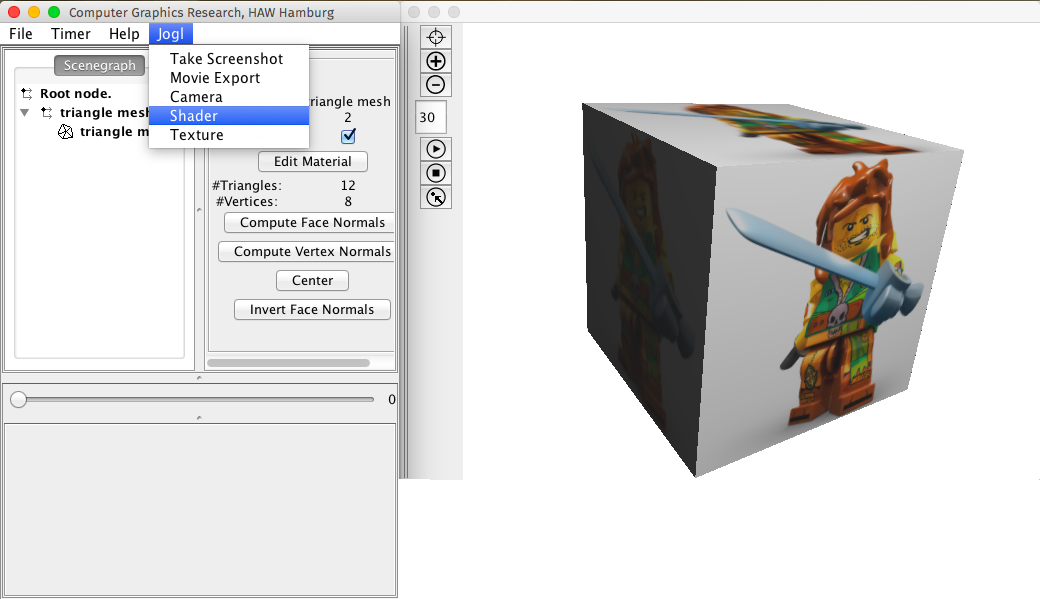
\includegraphics[height=8cm]{images/cgresearch.png}
\label{fig:cgapplication.png}
\caption{Screenshot einer Anwendung mit dem cgresearch Framework. Das Fenster besteht aus verschiedenen Bl�cken: 3D-View (rechts), Debug-Konsole (unten), Szenengraph und Controller (oben links) Editor-Dialoge (Mitte) und Men�.}
\end{figure} 

\subsection{Anwendungsobjekt}

In diesem Abschnitt wird beschrieben, wie mit dem cgresearch Framework eine Anwendung geschrieben werden kann. Als Rendering-System wird JOGL (siehe Abschnitte \ref{section:JOGL}) verwendet.

Im Zentrum einer Anwendung steht ein \verb+CgApplication+-Objekt. Darin spielt sich die eigentliche Logik der Anwendung ab. Zur Darstellung wird (optional) eine Instanz eines Rendering-Frames erzeugt. Auch das Benutzerinterface ist eine optionale Komponente. Die Klasse \verb+JoglSwingUserInterface+ stellt beispielsweise ein Benutzerinterface f�r das JOGL-System mit Java Swing bereit.

Die main-Methode der Anwendung k�nnte also lauten:
\begin{verbatim}
new ConsoleLogger(Logger.VerboseMode.DEBUG);
ResourcesLocator.getInstance().parseIniFile("resources.ini");
CgApplication app = new TriangleMeshFrame();
new JoglFrame(app);
new JoglSwingUserInterface(app);
\end{verbatim}
Zu dem Logger finden Sie Informationen im Abschnitt \ref{sec:logging}, der \verb+ResoucesLocator+ ist in Abschnitt \ref{section:ressourcen} dargestellt.

\subsection{Rendering}

Aktuell  stehen zwei Klassen (und damit Systeme) f�r das Rendering zur Verf�gung:
\begin{itemize}
\item \verb+JoglFrame+ (JOGL)
\item \verb+JMonkeyFrame+ (jMonkey)
\end{itemize}

Die Rendering-Systeme werden ausf�hrlicher in Abschnitt \ref{sec:rendering} besprochen.

\subsection{Grafische Benutzerschnittstelle}

Aktuell  stehen zwei Klassen (und damit Systeme) f�r das Benutzerinterface (UI) zur Verf�gung:
\begin{itemize}
\item \verb+SwingUserInterface+ (Java Swing)
\item \verb+JoglSwingUserInterface+ (Java Swing mit Zusatzfunktionalit�t f�r JOGL)
\end{itemize}

Die meisten Anwendungen werden durch ein grafisches Benutzerinterface (GUI) gesteuert. In einer Anwendung k�nnen Sie eigene Benutzerinterfaces umsetzen und registrieren. Diese tauchen dann als zus�tzlicher Tab im Fensterbereich \emph{Szenengraph und Controller} auf. Zum Schreiben eines solchen Controllers implementieren Sie eine eigene Klasse, die von der abstrakten Klasse \verb+IApplicationControllerGui+ erbt. Diese Klasse wiederum erbt von \verb+JPanel+. Sie m�ssen also das \verb+this+-Objekt mit Ihrem GUI bef�llen. Anschliessend registrieren Sie das Objekt bei Ihrer Instanz f�r die Grafische Benutzeroberf�che �ber die Methode \verb+registerApplicationGUI()+. Hier eine einfache Beispiel-Implementirerung f�r ein GUI, das aus einem Button besteht, der einen Tetraeder erzeugt:

\begin{verbatim}
public class PJController extends IApplicationControllerGui 
 	 	 	implements ActionListener {
 	public PJController() {
 	 	JButton button = new JButton("PJ!");
 	 	button.addActionListener(this);
 	 	add(button);
 	}

 	@Override
 	public String getName() {
 	 	return "PJ";
 	 }

 	@Override
 	public void actionPerformed(ActionEvent e) {
 	 	CgNode node = new CgNode(TriangleMeshFactory.createTetrahedron(), "Tetra");
 	 	getRootNode().addChild(node);
 	}
}
\end{verbatim}

\subsection{Men�s}

Ihre GUI-Anwendung kann auch um benutzerdefinierte Men�s erweitert werden. Das Vorgehen ist sehr �hnlich zum Vorgehen beim Erstellen einer eigenen GUI-Komponente aus dem vorherigen Abschnitt. Zun�chst muss eine Men�klasse implementiert werden, die von der abstrakten Klasse \verb+CgApplicationMenu+ abgeleitet ist. Diese Instanz registrieren Sie in Ihrer GUI-Instance: 
\begin{verbatim}
	registerApplicationMenu(new <Men�klasse>)); 
\end{verbatim}

Die Elternklasse der Men�klasse selber erbt von \verb+JMenu+. Daher m�ssen Sie einfach das \verb+this+-Objekt mit den gew�nschten Men�eintr�gen bef�llen, um ein Men� zu erstellen. Eine Beispielumsetzung einer Men�-Klasse ist:	

\begin{verbatim}
public class PjMenu extends CgApplicationMenu {
 	public MyMenu() {
 	 	super("MyMenu");
 	 	JMenuItem itemPrintMessage = new JMenuItem("Print message");
 	 	itemPrintMessage.addActionListener(new ActionListener() {
 	 	 	public void actionPerformed(ActionEvent e) {
 	 	 	 	System.out.println("Message");
 	 	 	}
 	 	});
 	 	add(itemPrintMessage);
 	}
}
\end{verbatim}


\subsection{Ressourcen}
\label{section:ressourcen}

An mehreren Stellen im cg-Framework wird auf Ressourcen aus dem Dateisystem zugegriffen (z.B. Icons, Bilder, Netze, Texturen, ...). Diese k�nnen sich in unterschiedlichen Pfaden befinden. Die Resourcenpfade werden zentral �ber eine Singleton-Klasse {\verb ResourcesLocator } verwaltet. In jedem Programm, das das Framework verwendet, muss daher der {\verb ResourcesLocator } mit den notwendigen Ressoucenpfaden gef�llt werden. Dazu stehen zwei Methoden zur Verf�gung: 

\begin{itemize}
	\item {\verb addPath(String) } Hinzuf�gen eines Pfades
	\item {\verb parseIniFile(String) } Lesen eine Liste von Pfaden (zeilenweise) aus einer INI-Datei
\end{itemize}

Alle Ressourcen, die intern geladen werden (z.B. Icons, Netze, Texturen), verwenden den {\verb ResourcesLocator }, um alle Resourcenpfade zu durchsuchen. Greift man in einem Anwendungsprogramm auch direkt auf Ressourcen zu, dann kann man die Methode {\verb getPathToResource(String) } verwenden. Diese liefert entweder einen g�ltigen Pfad f�r eine Resource oder null, falls die Ressource in keinem der Ressourcenpfade gefunden wurde.

Die Ressourcen, die direkt mit dem Projekt cgresearch bereitgestellt werden, befinden sich im Projektverzeichnis im Unterverzeichnis \emph{assets}.

\subsection{Logging}
\label{sec:logging}

Innerhalb des Frameworks wird ein konsistentes Logging-System verwendet. Der Logger ist als Singleton implementiert und kann folgendermassen erreicht werden:

\begin{verbatim}
Logger logger = Logger.getInstance();
\end{verbatim}

Dem Logger k�nnen folgende Nachrichten geschickt werden:

\begin{itemize}
\item \textbf{Nachricht:} Generelle Nachricht, wird normalerweise sofort ausgegeben
\item \textbf{Debug-Nachricht:} Debugging-Nachricht, wird normalerweise nur ausgegeben, wenn Debugging aktiviert ist
\item \textbf{Exception:} Auftritt einer Exception, wird normalerweise sofort ausgegeben.
\item \textbf{Error:} Auftritt eines Fehlers, wird normalerweise sofort ausgegeben.
\end{itemize}

Aktuell sind folgende Logger umgesetzt:

\begin{itemize}
\item \verb+ConsoleLogger+ Ausgabe auf der Konsole
\item \verb+LoggerPane+ Wird bei Verwendung der Swing-GUI angezeigt
\end{itemize}